\chapter{Care centers characterization}

\section{Motivation}

There are many care centers in France, which do not share the same degree of oncology specialization. Therefore, we first run a clustering algorithm to automatically group the care centers based on their medical statistics and attributes. Using these clusters, we label the care centers in terms of hospital development and oncology specialization.

\section{Methods}

\subsection{Data collection}

To run our method, it is necessary to gather data from multiple sources. There was no database already available that contained all the information we needed, so had to retrieve data from multiple locations and merge it. We first needed health data to characterize the care centers. Then, geographical and socio-demographic data was used to obtain information on the population locations.
Health data is collected from two sources: \ac{pmsi} and \ac{sae}. The \ac{pmsi} database is includes discharge summaries for all inpatients admitted to public and private hospitals in France. The \ac{sae} database is a compulsory and exhaustive administrative survey of all public and private hospitals in France. The survey is sent every year and describes the activities of the hospitals as well as the list of services and activities they provide. All the health statistics we used is for year 2018.
The list of hospitals in France is available in the \ac{pmsi} database and updated yearly. There were 5,148 hospitals in 2018. To obtain statistics on these care centers, we use the \ac{sae} database. There are more than 50 tables in the \ac{sae}. Only four tables were necessary. We start with the table "FILTRE" (n=4,041 hospitals) that gathers the general information about the hospital and the list of services it has. Then we use the "MCO" table (n=1,650 hospitals) which contains statistics on care centers with medical surgery or obstetric activity. The table "CANCERO" (997 hospitals) gathers statistics about oncology activity. Finally, the table "BLOCS" (1,057 hospitals) gathers information about surgery room activity.
We merge the care centers dataset extracted from the \ac{pmsi} with the \ac{sae} tables. "FINESS", "FILTRE" and "MCO" are merged with an inner join. This operation will remove care centers that do not declare MCO activity in the \ac{sae}. The tables "CANCERO" and "BLOCS" are merged with a left join, so that care center with no oncology or surgery activity could remain in the dataset. The missing values were filled with 0. The final merged dataset has 1,588 care centers.
Metropolitan France is divided into 13 regions, 96 departments, and around 35,000 municipalities. The number of municipalities changes each year but is roughly stable. Statistics on municipalities are publicly available on various governmental open data platforms. Municipalities and their census statistics are extracted from the \ac{insee} website. The most up to date data was re- leased in 2021: population data is from 2017 and 2012, socio-demographic data is from 2018. Municipalities latitude and longitude coordinates are retrieved from La Poste open data platform. In the \ac{pmsi} database, municipalities with small population are merged into "geographic codes", an aggregation of one or more municipalities. The list of the geo- graphic codes and the municipalities they are linked with are retrieved from the \ac{pmsi} database. We merge (inner join) the \ac{insee} dataset with coordinates extracted from La Poste and the geographic codes correspondence. After merging these tables, the final dataset comprises 13 regions, 96 departments, 34,877 municipalities and 5,608 geographic codes.

\subsection{Variable selection}

After the previous merge on the \ac{sae} health data, we had more than 200 variables for every care center. We selected a list of 24 variables with the help of medical experts. The variables are either binary when they encode the presence or absence of a service; or continuous when they encode the number of stays. Even though the "CANCERO" table gives us the number of stays related to oncology, we created a new variable to encode the oncology activity of a care center. Indeed, the number of stays for radiotherapy or chemotherapy is usually much higher than the number or surgery stays, resulting in an over-representation of these activities compared to surgery. The "CANCERO" table gives us the number of patients and the number of stays with radiotherapy and chemotherapy per care center. We subtracted the number of radiotherapy and chemotherapy stays from the number of oncology stays. We named this variable "CANCERO\_NB\_STAYS\_CHIRMED". Then we added to this the number of chemotherapy and radiotherapy patients, resulting in a new variable that we refer as "ONCOLOGY\_ACTIVITY". Finally, log transformation is applied to continuous data and standard scaling (0 mean and unit variance) on every variable. The list of variables and their description are listed in \cref{table:sae-variables}.

\begin{table}[H]
    \centering
    \resizebox{\textwidth}{!}{%
        \begin{tabular}{|l|l|l|l|}
        \hline
            \acs{sae} table & Variable name & Variable definition & Distribution \\ \hline
            FILTRE & CHIRAMBU & Outpatient surgery activity & Binary \\ \hline
            FILTRE & CHIMIO & Chemotherapy activity & Binary \\ \hline
            FILTRE & RTH & Radiotherapy activity & Binary \\ \hline
            FILTRE & BLOC & Surgery activity & Binary \\ \hline
            FILTRE & BIO & Medical biology or anatomopathological activity & Binary \\ \hline
            FILTRE & REA & Intensive care unit & Binary \\ \hline
            FILTRE & MEDIC & Medication circuit & Binary \\ \hline
            FILTRE & DOULEUR & Chronic pain & Binary \\ \hline
            FILTRE & PALIA & Palliative care & Binary \\ \hline
            FILTRE & CHIRCANCER & Cancer surgery & Binary \\ \hline
            \acs{mco} & SEJHC\_MED & Number of inpatient medical stays & Continuous \\ \hline
            \acs{mco} & SEJHC\_CHI & Number of inpatient surgery stays & Continuous \\ \hline
            \acs{mco} & SEJHP\_MED & Number of outpatient medical stays & Continuous \\ \hline
            \acs{mco} & SEJHP\_CHI & Number of outpatient surgery stays & Continuous \\ \hline
            \acs{mco} & LIT\_MCO & Number of \acs{mco} beds & Continuous \\ \hline
            BLOCS & SALCHIR & Number of surgery operating rooms & Continuous \\ \hline
            BLOCS & SALAMBU & Operating rooms dedicated to outpatient surgery & Continuous \\ \hline
            CANCERO & CANCERO\_A1 & Use chemotherapy for cancer treatment & Binary \\ \hline
            CANCERO & CANCERO\_A2 & Use radiotherapy for cancer treatment & Binary \\ \hline
            CANCERO & CANCERO\_A3 & Has an oncology dedicated unit & Binary \\ \hline
            CANCERO & CANCERO\_A11 & Number of patients treated with chemotherapy & Continuous \\ \hline
            CANCERO & CANCERO\_A17 & Number of patients treated with radiotherapy & Continuous \\ \hline
            - & CANCERO\_NB\_STAYS\_CHIRMED & Number of oncology medical or surgery stays  & Continuous \\ \hline
            - & CANCERO\_ACTIVITY & Oncology activity & Continuous \\ \hline
        \end{tabular}}
    \caption{
        \textbf{List of the variables used for clustering, and their definitions.} All the variables except CANCERO\_NB\_STAYS\_CHIRMED and CANCERO\_ACTIVITY are coming from \ac{sae}. The variables are either binary or continuous. Oncology activity is the sum of CANCERO\_NB\_STAYS\_CHIRMED, CANCERO\_A17 and CANCERO\_A11.
    }
    \label{table:sae-variables}
\end{table}

\subsection{\acf{pca}}

\ac{pca} is dimensionality-reduction method. It is used to reduce the dimensionality of large data sets, by transforming a large set of variables into a smaller one. The new dataset still contains most of the information in the large set. Dimensionality reduction trades accuracy for simplicity and has multiple ad- vantages. First, dimensionality reduction removes redundant and highly correlated features. Then training statistical models on reduced data is easier and less computation- ally expensive. Moreover, dimensionality reduction makes it possible to visualize large dimensional data. In practice, \ac{pca} projects the original data onto new directions, referred as components. Each component explains some of the variance from the original dataset. Keeping the $n$ components with maximum variance and dropping the other ones performs the actual dimensionality reduction. We call "explained variance" the sum of the variance explained by the components kept. \ac{pca} is relatively easy to interpret, as each component is a linear combination of the input variables. The contributions of each input variable to the \ac{pca} components are called loading scores.
We apply the \ac{pca} algorithm to the SAE dataset that describes the care centers. We used Python's scikit-learn \cite{pedregosa_scikit-learn_2011} implementation of the \ac{pca}, since it's very well documented and maintained. The input data has 24 variables, and we perform a dimensionality reduction with $n=2$ components. We tried different number of components, from 2 to 5, but we found 2 gave good and easy to interpret results.

\subsection{Clustering}

Clustering is the task of grouping data points in such a way that points in the same group are closer to each other than to those in other groups. It is an unsupervised Machine Learning algorithm and does not need labelled data to train on. There are different types of clustering methods and different algorithms. Hard clustering is when each point belongs to a cluster or not. Soft clustering is when each point belongs to each cluster to a certain degree. There are many clustering algorithms, Xu and Tian wrote a comprehensive survey on them \cite{xu_comprehensive_2015}. We want to run a clustering algorithm on the \ac{pca} reduced dataset to automatically isolate care centers with similar statistics. We tried several algorithms, and, in our case, Spectral Clustering \cite{luxburg_tutorial_2007} worked best. Again, we used Python's scikit-learn Machine Learning library \cite{pedregosa_scikit-learn_2011} since they implemented most of the widely known clustering algorithms. The number $k$ of clusters is a hyper parameter and there is no universal rule to select the best number. We tried various values from 2 to 10 and manually interpreted the results with medical experts. We found that 8 clusters gave the most interpretable groups. The \ac{pca} and clustering results are visible on \cref{fig:clustering-pca}.

\begin{figure}[H]
    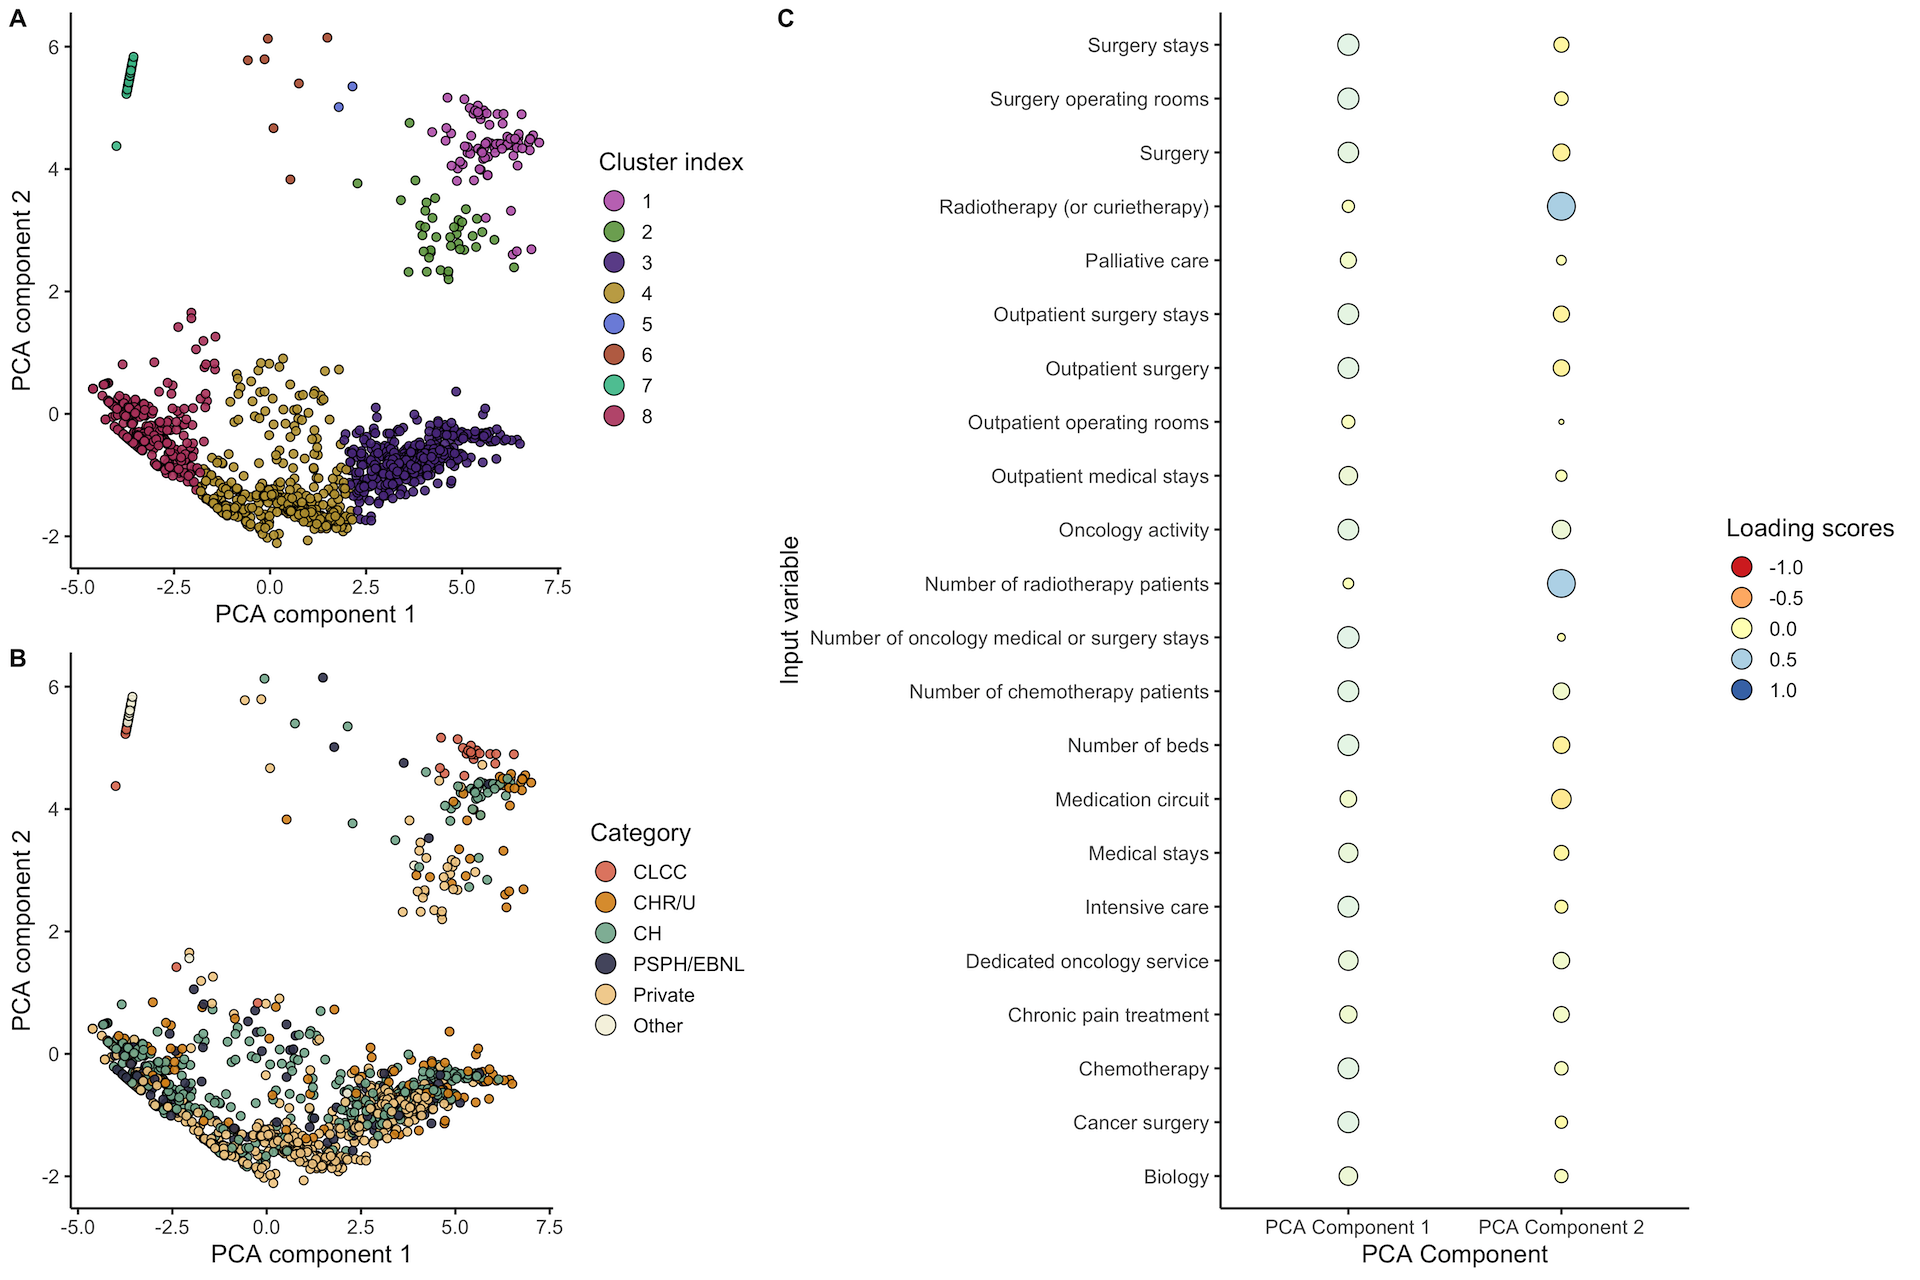
\includegraphics[width=\textwidth]{images/camion/supplemental/sup_fig1_pca_and_clustering.png}
    \centering
    \caption{
        \textbf{\ac{pca} interpretation}. Care centers are showed as points in the 2-dimensional \ac{pca} space. Points are colored by cluster index (A) and hospital type (B). \ac{clcc} care centers are close together in the \ac{pca} space, proving they have similar activity and services distribution. \ac{pca} components are a linear combination of the input variables (C). The loading scores reflect how much the input variable contributed to the \ac{pca} component. Component 1 is associated with most of the variables, while component 2 is linked with radiotherapy variables. Hence, we interpret component 1 as hospital size and component 2 as oncology specialization.
    }
    \label{fig:clustering-pca}
\end{figure}

\section{Results}

In 2018, the population in France was 66,993 million. Mainland France hosts 64,812 million inhabitants (96.8\%), while the remaining 2,181 million (3.2\%) live in overseas departments and regions . Metropolitan France is divided into 13 administrative regions and 96 departments. The population density in France is unevenly distributed . In 2020, the overall population density in metropolitan France was 119 inhabit-ants per square kilometer. Ile-de-France region has the highest population density with 1,022 inhabitants per square kilometer. Density in other regions in metropolitan France range between 40 and 187 inhabit-ants/km2. Denser areas are located near the coastline and around the largest cities like Paris, Marseille, Lyon, Strasbourg, Toulouse, or Bordeaux. The middle of the country is rural, and the population densities are low. While there are a great variety of regions and landscapes, the country is becoming more urbanized. This ``rural exodus'' is largely responsible of what is known as the ``empty diagonal'', a band of very low-density population that stretches from the southwest to the northeast.
We now describe the spatial distribution and specificities of the 1,662 hospitals included in this study. There are different types of hospitals in France: \ac{ch}  (n=667) and \ac{chru}  (n=142) are state-run hospitals; \ac{clcc}  (n=26) and \ac{psph}/\ac{ebnl}  (n=142) are both private hospitals of collective interest, though \ac{clcc} are oncology dedicated; private hospitals (n=606) are privately run and for-profit. The non \ac{mco} care centers with radiotherapy activity (n=79) are mostly private practice structures and are referred as “Other”. \cref{table:oncology-activity-per-region} shows the number of care centers and their oncology activity per hospital type and region. Most of the care centers are public, but a non-insignificant part are private. \ac{clcc} rep-resent only 1.6\% of the care centers, yet they are responsible for 14.2\% of the overall oncology activity. The care centers are unevenly distributed across the country. For instance, Corse and Centre-Val-de-Loire are the only two regions with no \ac{clcc} care centers. Moreover, the proportion of oncology activity per hospital type varies from a region to another. For instance, in Nouvelle-Aquitaine, 47.1\% of the oncology activity is handled by private care centers, whereas in Provence-Alpes-Cote-d'Azur it is 21.4\%.

While it is obvious that \ac{clcc} care centers are suited for oncology care, it is difficult to assess the degree of oncology specialization for other care centers. Our clustering algorithm assigns the n=1,662 care centers into 8 clusters, sorted by oncology specialization. \cref{fig:clustering-spider} shows the distribution of some of the key health services per cluster. These services are biology, radio-therapy, chemotherapy, cancer surgery, intensive unit, palliative care, oncology unit, medication circuit, surgery, and outpatient surgery. The three oncology services are cancer surgery, radiotherapy, and chemo-therapy. We see that care centers from clusters 1 (n=79) and 2 (n=39) all have these 3 services, hence they are the most suited hospitals for oncology care. Centers from cluster 3 (n=451) have cancer surgery and chemotherapy but lack radiotherapy. The most part of the n=381 centers from cluster 4 have cancer surgery, but no radiotherapy nor chemotherapy. Care centers from cluster 5 (n=2) and cluster 6 (n=7) have radio-therapy and chemotherapy services, but no cancer surgery. Care centers in cluster 7 (n=77) are dedicated to radiotherapy and mostly private practice structures. Finally, care centers 8 (n=626) have none of the 3 oncology services. To sum up, hospitals from clusters 1 and 2 (n=118) are “all-in-one” care centers that provide the most “ideal” oncology care. Centers from clusters 3 and 4 (n=382) provide oncology care but will have to be coordinated with additional structures during the pathways. Hospitals within clusters 5, 6 and 7 (n=86) are not allowed to perform cancer surgery but pro-vide chemotherapy or radiotherapy. The remaining n=626 care centers in cluster 8 are not equipped for oncology care.

\begin{figure}[H]
    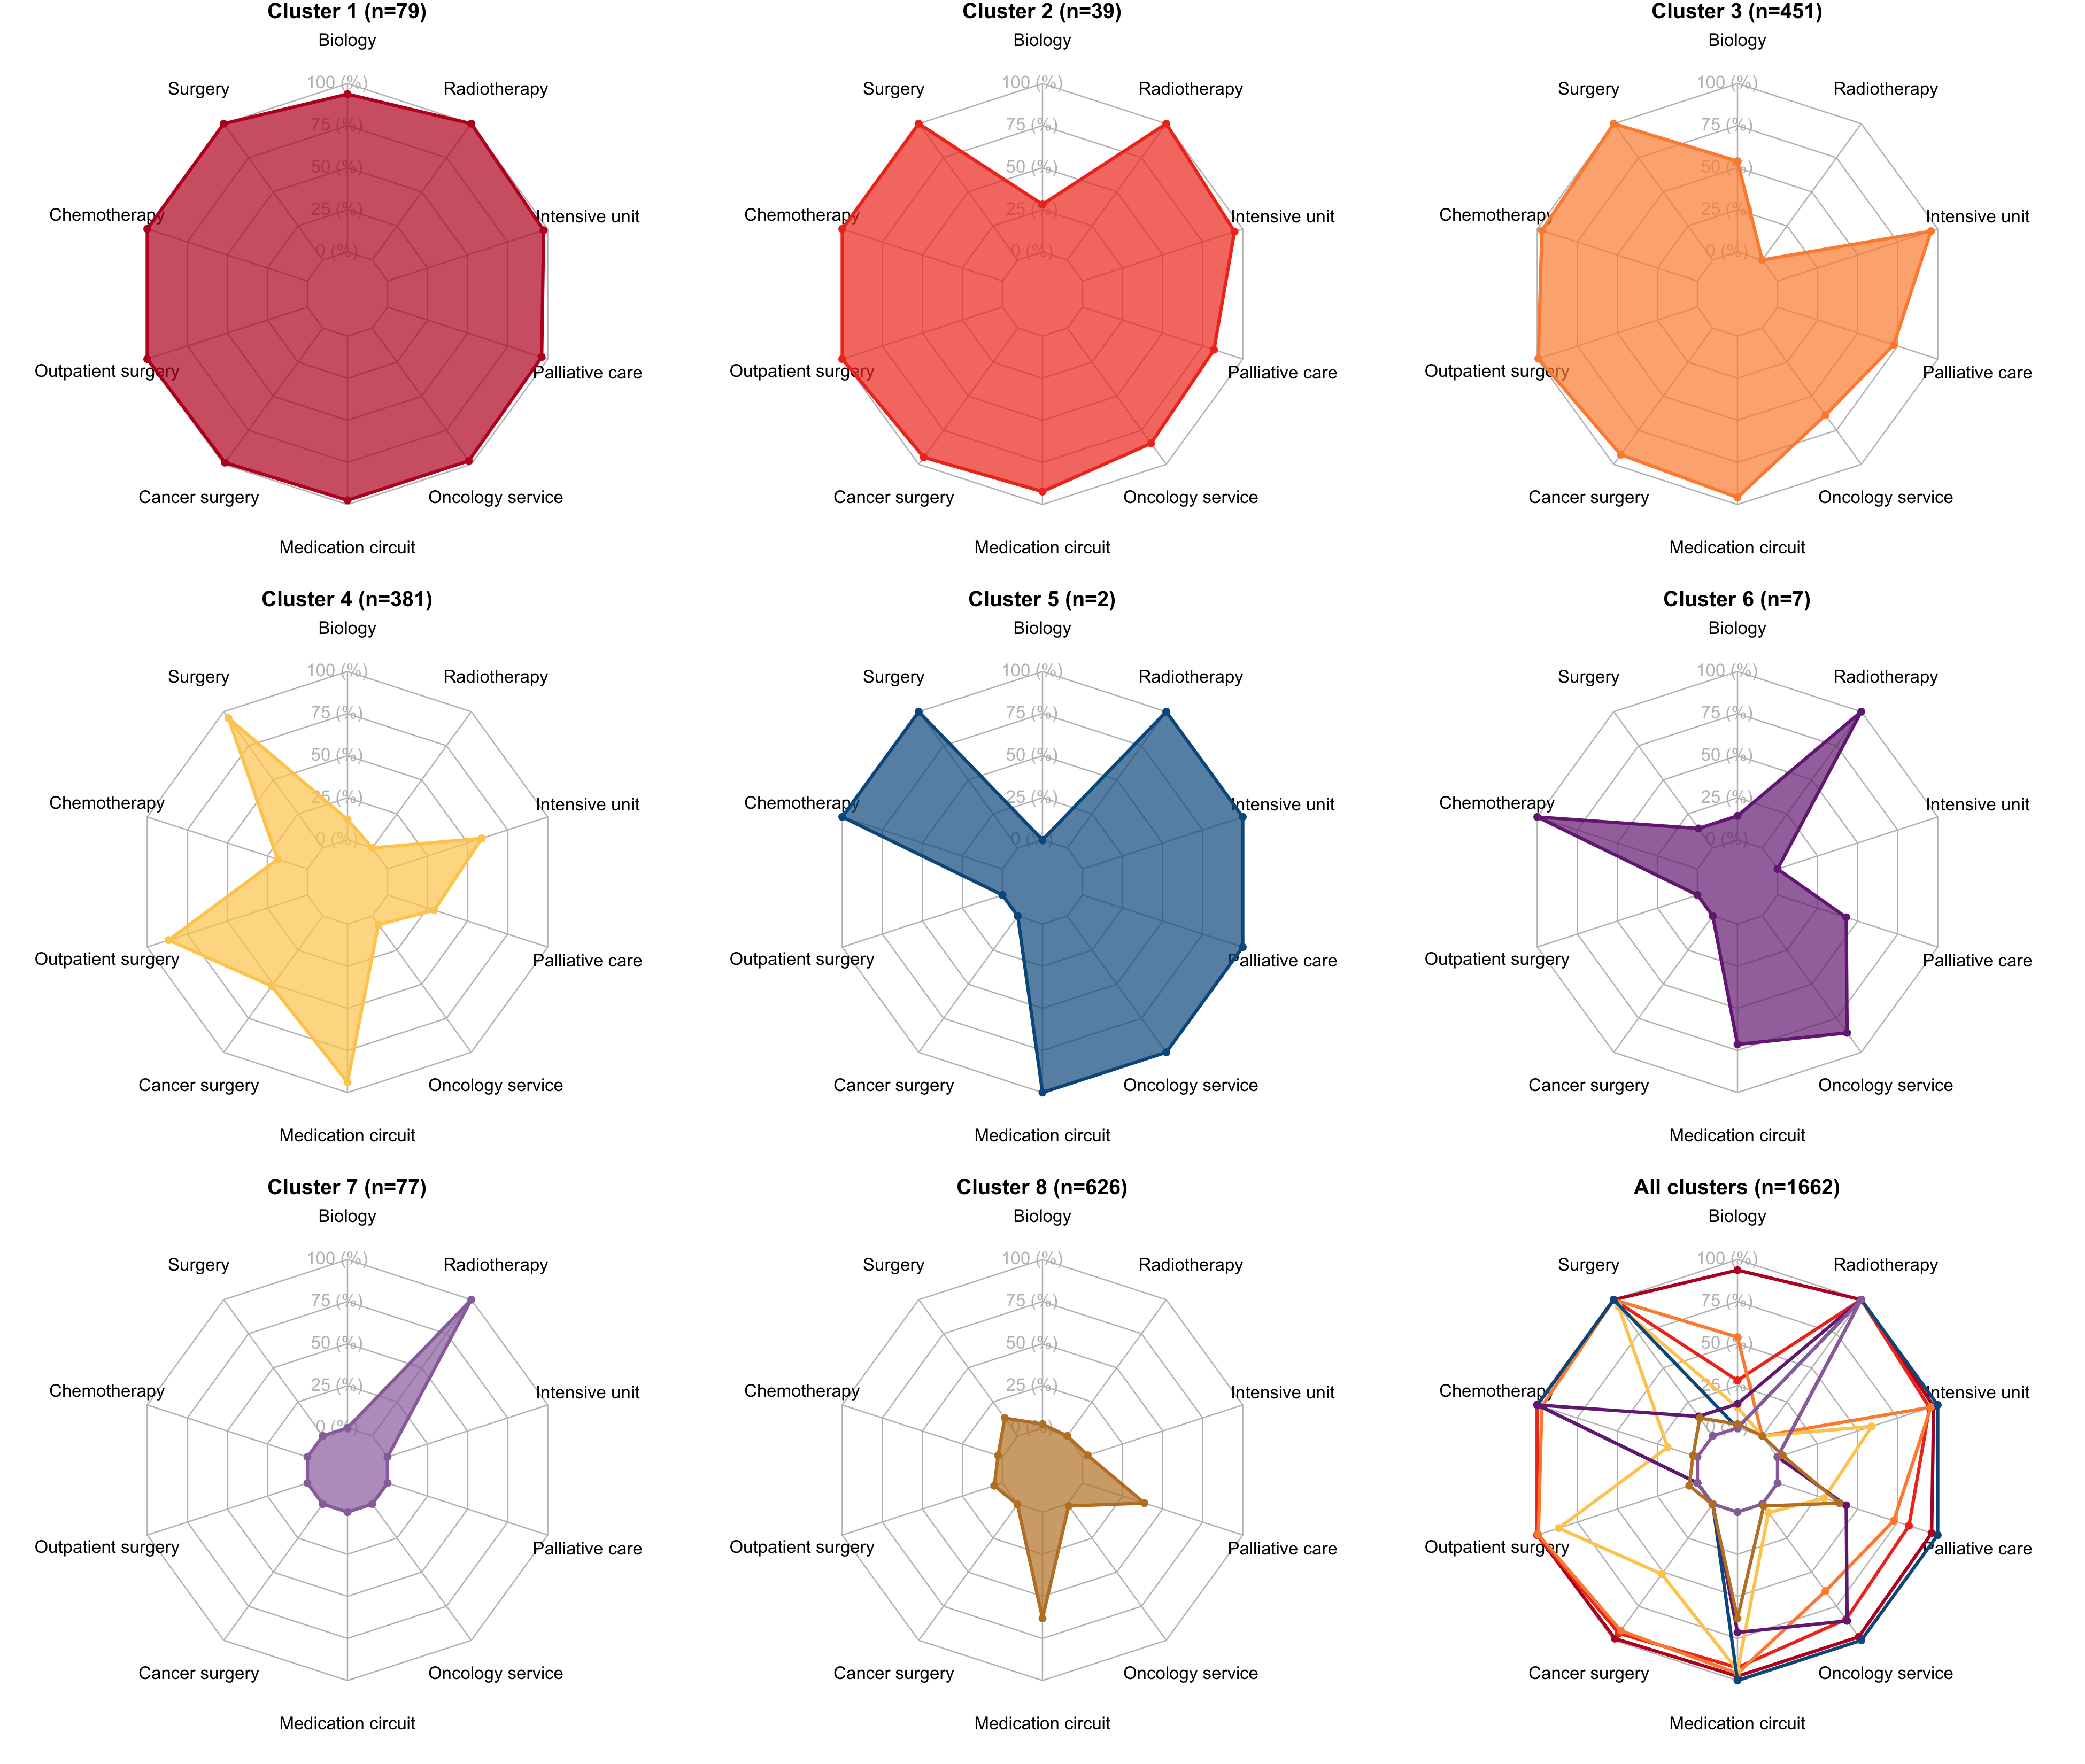
\includegraphics[width=\textwidth]{images/camion/fig1_clusters_services.png}
    \centering
    \caption{
        \textbf{Distribution of the care centers services and equipment per cluster.} Each radar plot axis shows the percentage of the care centers within the cluster that have the corresponding attribute. In Cluster 1, the care centers have all the listed services. In cluster 8, the centers have almost none of the services. Care centers from cluster 1 (n=79) and cluster 2 (n=39) are the most suit-ed for oncology care.
    }
    \label{fig:clustering-spider}
\end{figure}

Hospital types are unevenly distributed among the clusters as illustrated on \cref{fig:clustering-categories}. For instance, 76.9\% of the \ac{clcc} care centers are placed in cluster 1, as they are the most specialized centers. In cluster 7, we find external radiotherapy units of some \ac{clcc} centers, and private practice structures. The proportion of private care centers varies as well: cluster 1 has almost no private care center while cluster 2 has 61.5\% of private hospitals.

\begin{figure}[H]
    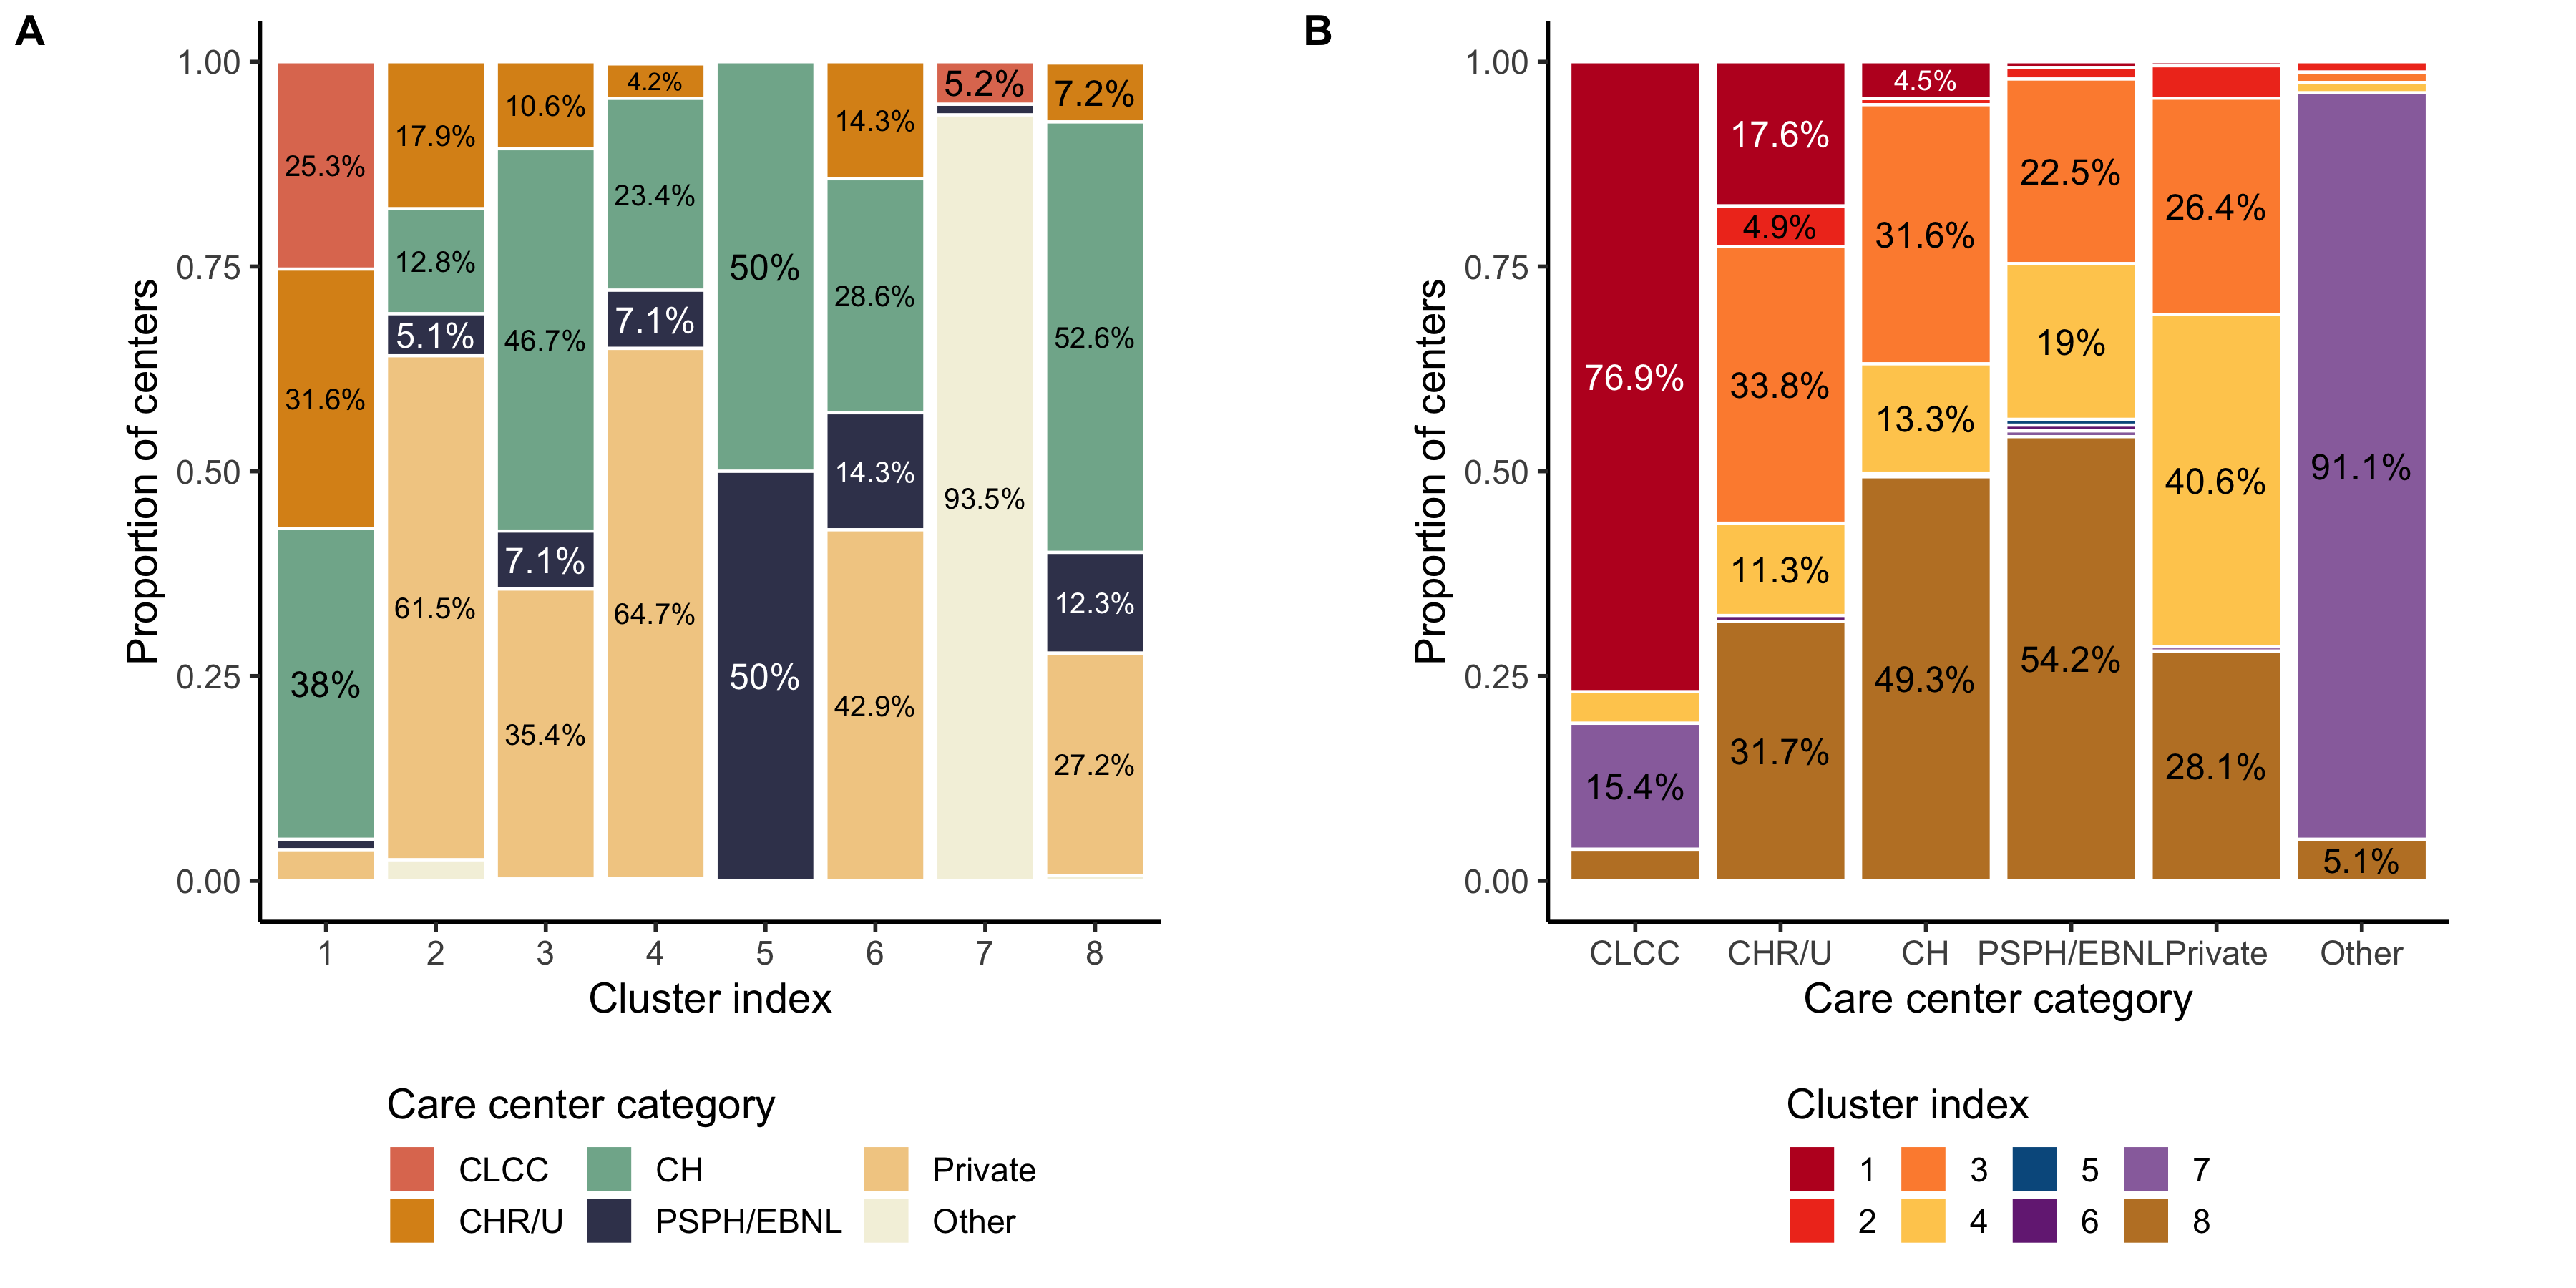
\includegraphics[width=\textwidth]{images/camion/supplemental/sup_fig2_categories_per_cluster.png}
    \centering
    \caption{
        \textbf{Comparison between hospital types and assigned clusters.} The majority of the \ac{clcc} care centers are grouped together in cluster 1. Moreover, cluster 1 has a very low percentage of private hospitals, whereas this proportion is the much higher in cluster 2. “Other” care centers are mostly private practice radiotherapy struc-tures, and they are regrouped in cluster 7.
    }
    \label{fig:clustering-categories}
\end{figure}

Moreover, most of the oncology activity is handled by care centers from clusters 1 and 3, as seen on \cref{fig:clustering-cumulative}. Also, the overall oncology activity from the n=79 centers in cluster 1 is almost as large as the activity of the n=451 hospitals from cluster 4.

\begin{figure}[H]
    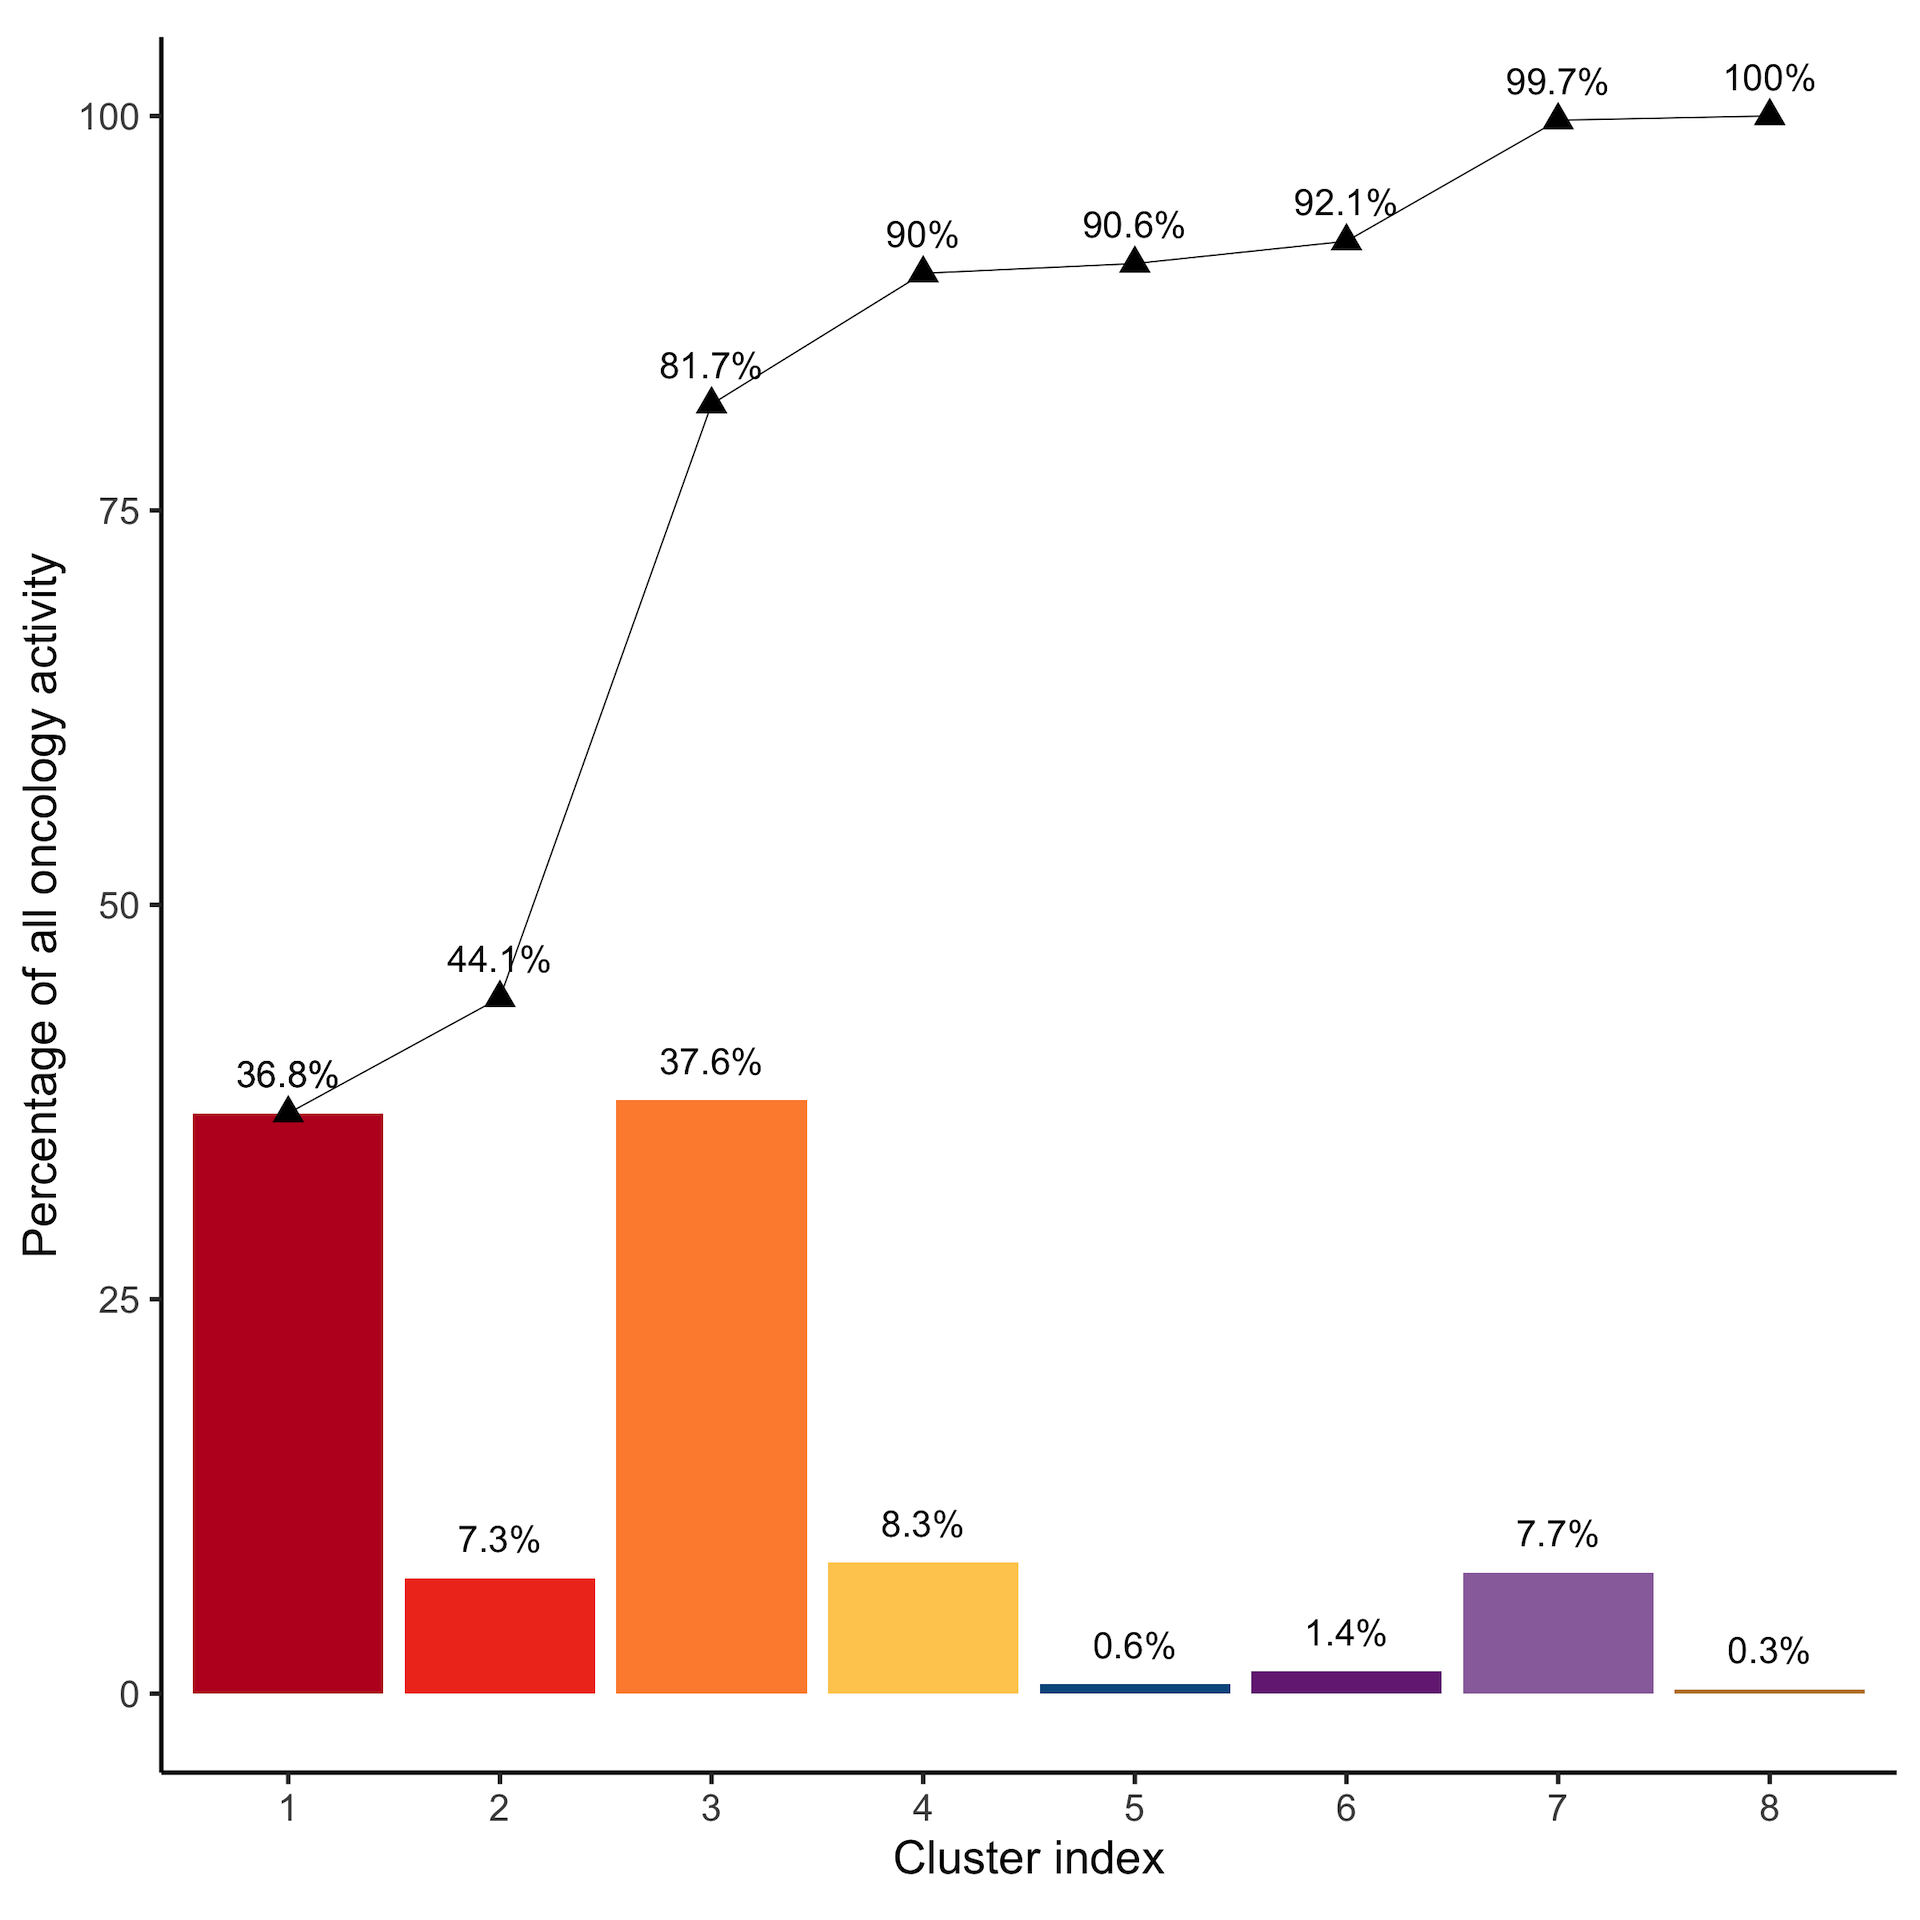
\includegraphics[width=0.5\textwidth]{images/camion/supplemental/sup_fig3_nb_stays_per_cluster.png}
    \centering
    \caption{
        \textbf{Cumulative sum of the oncology activity, per cluster.} Most of the oncology activity is handled by care centers from clusters 1 and 3. While there are only n=79 care centers in cluster 1, their total activity is almost as large as the n=451 care centers from cluster 3.
    }
    \label{fig:clustering-cumulative}
\end{figure}

\begin{figure}[H]
    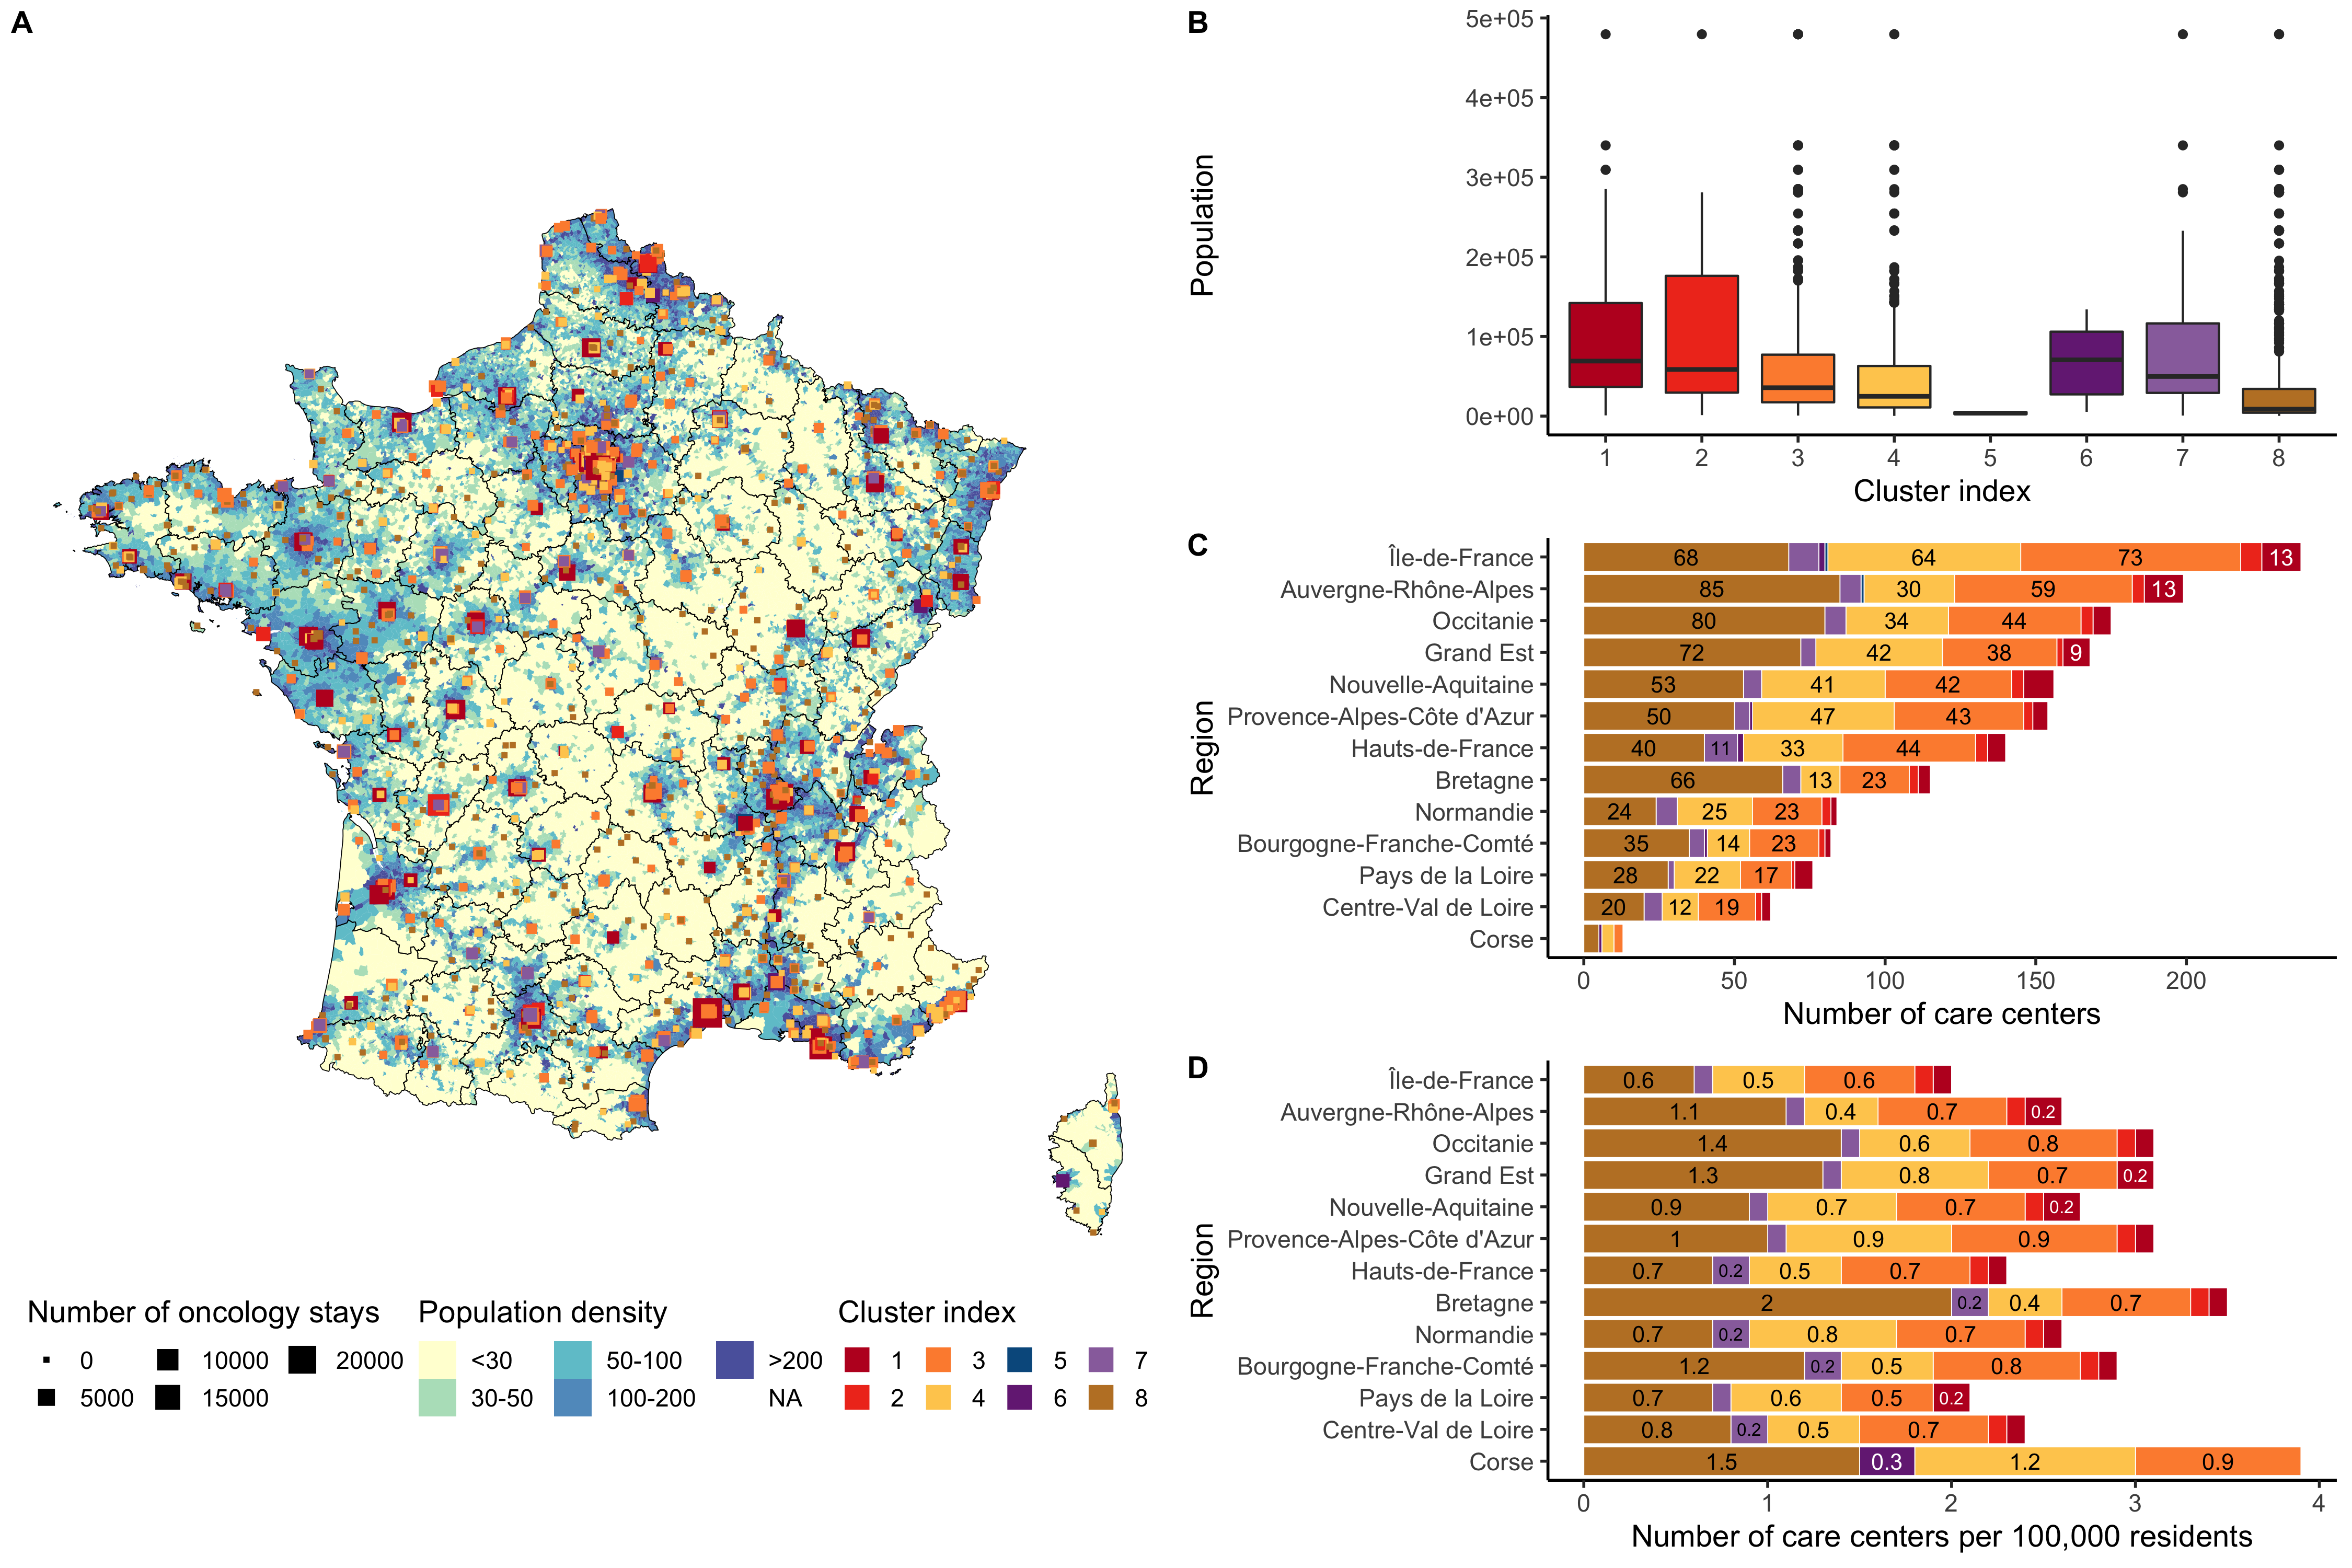
\includegraphics[width=\textwidth]{images/camion/supplemental/sup_fig4_care_centers_pop_density.png}
    \centering
    \caption{
        \textbf{Care centers spatial distribution, compared with population density.} Population density in metropolitan France is unevenly distributed across the country (A). Areas in the middle, near the Pyrenees and the Alps have very low population densities. The most specialized care centers are in dense areas and in large municipalities (B). While Ile-de-France has the highest number of care centers, it has the least care centers per 100,000 habit-ants.
    }
    \label{fig:clustering-map}
\end{figure}

\begin{table}[H]
    \resizebox{\textwidth}{!}{%
    \begin{tabular}{|l|l|l|l|l|l|l|l|l|}
    \hline
        Variable value per region & ~ & \multicolumn{7}{c}{Hospital Type} \\ \hline
        N = number of centers & ~ & \acs{ch} & \acs{ch} & \acs{clcc} & Other & \acs{psph}/\acs{ebnl} & Privé & All \\
        A = oncology activity (radio. + chemo. + surgery) & ~ &  (n=667)  & (n=142) & (n=26) & (n=79) & (n=142) & (n=606) & n=1,662 \\ \hline
        Auvergne-Rhône-Alpes & N & 98 (49,2\%) & 21 (10,6\%) & 2 (1\%) & 7 (3,5\%) & 13 (6,5\%) & 58 (29,1\%) & 199 \\
        ~ & A & 34,597 (26,7\%) & 31,706 (24,5\%) & 16,966 (13,1\%) & 6,710 (5,2\%) & 6,146 (4,7\%) & 33,297 (25,7\%) & 129.422 \\ \hline
        Bourgogne-Franche-Comté & N & 53 (64,6\%) & 4 (4,9\%) & 1 (1,2\%) & 5 (6,1\%) & 2 (2,4\%) & 17 (20,7\%) & 82 \\
        ~ & A & 12,238 (27,6\%) & 10,621 (24\%) & 5,844 (13,2\%) & 4,405 (9,9\%) & 657 (1,5\%) & 10,571 (23,8\%) & 44.336 \\ \hline
        Bretagne & N & 38 (33\%) & 8 (7\%) & 1 (0,9\%) & 6 (5,2\%) & 11 (9,6\%) & 51 (44,3\%) & 115 \\
        ~ & A & 15,953 (27\%) & 11,020 (18,6\%) & 6,341 (10,7\%) & 5,553 (9,4\%) & 2,050 (3,5\%) & 18,199 (30,8\%) & 59.116 \\ \hline
        Centre-Val de Loire & N & 29 (46,8\%) & 4 (6,5\%) & 0 (0\%) & 6 (9,7\%) & 2 (3,2\%) & 21 (33,9\%) & 62 \\
        ~ & A & 6,989 (19,6\%) & 11,524 (32,2\%) & 0 (0\%) & 5,137 (14,4\%) & 32 (0,1\%) & 12,058 (33,7\%) & 35.74 \\ \hline
        Corse & N & 7 (53,8\%) & 0 (0\%) & 0 (0\%) & 0 (0\%) & 0 (0\%) & 6 (46,2\%) & 13 \\
        ~ & A & 3,486 (66,3\%) & 0 (0\%) & 0 (0\%) & 0 (0\%) & 0 (0\%) & 1,773 (33,7\%) & 5.259 \\ \hline
        Grand Est & N & 70 (41,7\%) & 17 (10,1\%) & 3 (1,8\%) & 6 (3,6\%) & 30 (17,9\%) & 42 (25\%) & 168 \\
        ~ & A & 17,428 (19,6\%) & 22,123 (24,9\%) & 13,176 (14,8\%) & 6,793 (7,7\%) & 7,683 (8,7\%) & 21,553 (24,3\%) & 88.756 \\ \hline
        Hauts-de-France & N & 56 (40\%) & 11 (7,9\%) & 1 (0,7\%) & 11 (7,9\%) & 12 (8,6\%) & 49 (35\%) & 140 \\
        ~ & A & 21,864 (26\%) & 15,934 (19\%) & 6,947 (8,3\%) & 8,618 (10,3\%) & 5,242 (6,2\%) & 25,399 (30,2\%) & 84.004 \\ \hline
        Île-de-France & N & 40 (47,6\%) & 5 (6\%) & 4 (4,8\%) & 6 (7,1\%) & 3 (3,6\%) & 26 (31\%) & 84 \\
        ~ & A & 7,573 (14,9\%) & 7,947 (15,7\%) & 14,210 (28\%) & 5,419 (10,7\%) & 0 (0\%) & 15,627 (30,8\%) & 50.776 \\ \hline
        Normandie & N & 70 (44,9\%) & 10 (6,4\%) & 1 (0,6\%) & 7 (4,5\%) & 12 (7,7\%) & 56 (35,9\%) & 156 \\
        ~ & A & 37,844 (33\%) & 26,244 (22,9\%) & 7,477 (6,5\%) & 7,157 (6,2\%) & 2,824 (2,5\%) & 33,271 (29\%) & 114.817 \\ \hline
        Nouvelle-Aquitaine & N & 66 (37,7\%) & 14 (8\%) & 2 (1,1\%) & 7 (4\%) & 6 (3,4\%) & 80 (45,7\%) & 175 \\
        ~ & A & 14,735 (12,1\%) & 20,915 (17,2\%) & 16,047 (13,2\%) & 11,572 (9,5\%) & 1,098 (0,9\%) & 57,374 (47,1\%) & 121.741 \\ \hline
        Occitanie & N & 34 (44,7\%) & 5 (6,6\%) & 3 (3,9\%) & 4 (5,3\%) & 5 (6,6\%) & 25 (32,9\%) & 76 \\
        ~ & A & 11,901 (18,9\%) & 11,374 (18,1\%) & 12,564 (19,9\%) & 3,422 (5,4\%) & 3,916 (6,2\%) & 19,822 (31,5\%) & 62.999 \\ \hline
        Pays de la Loire & N & 53 (34,4\%) & 10 (6,5\%) & 3 (1,9\%) & 4 (2,6\%) & 15 (9,7\%) & 69 (44,8\%) & 154 \\
        ~ & A & 14,632 (13,6\%) & 16,533 (15,4\%) & 21,924 (20,4\%) & 6,172 (5,7\%) & 10,918 (10,2\%) & 37,176 (34,6\%) & 107.355 \\ \hline
        Provence-Alpes-Côte d'Azur & N & 53 (22,3\%) & 33 (13,9\%) & 5 (2,1\%) & 10 (4,2\%) & 31 (13\%) & 106 (44,5\%) & 238 \\
        ~ & A & 24,390 (12,6\%) & 66,406 (34,2\%) & 34,028 (17,5\%) & 12,817 (6,6\%) & 14,981 (7,7\%) & 41,577 (21,4\%) & 194.199 \\ \hline
        Grand Total & N & 667 (40,1\%) & 142 (8,5\%) & 26 (1,6\%) & 79 (4,8\%) & 142 (8,5\%) & 606 (36,5\%) & 1662 \\
        ~ & A & 223,630 (20,4\%) & 252,347 (23\%) & 155,524 (14,2\%) & 83,775 (7,6\%) & 55,547 (5,1\%) & 32,7697 (29,8\%) & 1,098,520 \\ \hline
    \end{tabular}}
    \caption{
        \textbf{Number of care centers (N) and overall oncology activity (A) per hospital type and region.} Oncology activity is the sum of the number of patients with radiotherapy or chemotherapy, and the number of medical or surgery stays related to cancer. \ac{ch} and \ac{ch} are public hospitals; \ac{clcc} and \ac{psph}/\ac{ebnl} are private hospitals of collective interest, though \acs{clcc} are oncology dedicated; private hospitals are for-profit. “Other” hospitals are mostly private practice radiotherapy structures. The percentages sum to 100\% row-wise. In Nouvelle-Aquitaine, 47.1\% of the oncology activity is handled by private care centers, whereas in Provence-Alpes-Cote-d’Azur it is 21.4\%.
    }
    \label{table:oncology-activity-per-region}
\end{table}

\section{Discussion}

The clustering algorithm successfully groups similar hospitals and lets us identify the care centers best suited for oncology care. Some variables in the \ac{sae} survey are declarative and potentially differ from the reality. We are aware of this bias, but we do not expect major differences that could distort our clustering results.
Receiving treatment in a care center with surgery, chemotherapy and radiotherapy activities is easier for the patient and leads to better care pathways. Care centers from cluster 1 will be the better choice for cancer treatment and correspond to modern oncology care specifications. However, these centers are a minority and sparsely located, essentially in dense areas and in large cities. While the inhabitants of large cities and metropolitan areas will have no problem reaching them, rural areas residents live far away from these centers. This population often has better access to care centers from intermediate clusters. Such centers do not have all the key services and the patients are more likely to visit multiple hospitals during their care pathways.
Longer drives to reach a more specialized care center could be considered more acceptable for surgery, where the hospital volume and surgeon expertise matter. However, for more frequent interventions like chemotherapy and radiotherapy especially, patients should prioritize short travels. There is a tradeoff to be found by patients, between care center proximity and care center expertise. This dilemma will be more frequent for patients living in rural areas than patients living in dense cities with large care centers nearby.

